
\section{Datasets}

In our approach we propose a supervised machine learning algorithm to estimate the page rank using deep graph networks. For this purpose we require labeled data to develop, train, and validate our model. Each dataset version was created to answer a specific question raised during our research.

All dataset versions have OpenPage Rank (\ref{OpenPageRank}) as ground truth. Ground truth means in our case that we use the ordered list of domains from OpenPage Rank in the datacrawler to enrich them with more information thus to generate our datasets.

The following sections will profoundly discuss each dataset and the questions answered. 

\subsection{Dataset Version 1}
\label{DatasetVersion1}
The goal of the dataset version 1 was to answer the question on how well CNNs perform on estimating a page rank of a website. The provided data was used to train a CNN and evaluate his performance on page rank estimation.

The dataset version 1 consists of 100,000 samples in total. Every sample $X$ corresponds to a domain $x$ contained in the ground truth. We denote the $r^{th}$ sample as $x^{(r)}$ in the ground truth and $X^{(r)}$ in the dataset. 
A single sample in the ground truth can be expressed as a tuple consisting of two values:

\begin{center}
	$x^{(r)} = (r, u)$
	\begin{itemize}
		\item[$r$] The global rank of the domain, according to Open PageRank, within $[1, 100000]$. 
		\item[$u$] The URL of the domain. For example a string like \texttt{github.com}.
	\end{itemize}
\end{center}

A single sample in the dataset can be expressed as a tuple consisting of three values:

\begin{center}
 $X^{(r)} = (\tensorsym{I}, r, u)$
\begin{itemize}
	\item[$\tensorsym{I}$] The screenshot of the domain in image format PNG and in the resolution $1920\times1080$. The screenshot is generated by the datacrawler for the given domain corresponding to the ground truth. The image tensor has four channels, each representing a channel of the color space RGBA. Thus, a screenshot can be represented as $\tensorsym{I}\in[0,255]^{1920\times1080\times4}$. For ensuring repeatability, only the upper visible area of the website has been taken into account, which is provided during the initial visit of the website. 
	\item[$r$] The global rank of the domain, according to Open PageRank, within $[1, 100000]$. 
	\item[$u$] The URL of the domain mapped by the Open PageRank list. For example a string like \texttt{github.com}.
\end{itemize}
\end{center}

\subsection{Dataset Version 2}
\label{DatasetVersion2}
\subsubsection{Overview}
The goal of the dataset version 2 is to enable the subject of our research the evaluation of deep graph networks for page rank estimation. The provided data was used to train and evaluate deep graph networks.

There are in total 100,000 samples in dataset version 2. Like dataset version 1, every sample $X$ corresponds to a domain $x$ contained in the ground truth. Moreover we denote the $r^{th}$ sample as $x^{(r)}$ in the ground truth and $X^{(r)}$ in the dataset as well. 
But unlike dataset version 1, a single sample in the dataset version 2 is a tuple consisting of four values:

\begin{center}
$X^{(r)} = (G,u,r,h)$
\begin{itemize}
    \item[$G$] The directed graph of the domain characterized by a set of nodes $\mathbb{V}$ and edges $\mathbb{E}$: $G= \left(\mathbb{V}, \mathbb{A}\right)$. The directed graph $G$ (\ref{TheDirectedGraph}) is generated by the datacrawler for the given domain corresponding to our ground truth.
	\item[$u$] The URL of the domain mapped by the Open PageRank list.
	\item[$r$] The global rank of the domain, according to Open PageRank, within $[1, 100000]$. 
    \item[$h$] Indicator for whether or not the website uses the protocol HTTPS, the value is $\in\left\{\text{true}, \text{false}\right\}$.
\end{itemize}
\end{center}

\subsubsection{The Directed Graph $G$}
\label{TheDirectedGraph}
The directed graph provides a topological view on the given website by representing all associated web pages within the same domain as vertices and connections as arrows. Figure \ref{fig:PartialDirectedGraph_timodenk.com} illustrates this by means of an example. During the crawling process as described in Section \ref{Datacrawler} vertices and arrows of the graph are created and enriched with local information about the visited web pages.

The directed graph $G$ is characterized by a set of nodes $\mathbb{V}$ and edges $\mathbb{E}$. Each node $v \in \mathbb{V}$ represents a web page of the given domain associated with the graph. A node is characterized by the following tuple:

\begin{center}
$v = (u, \tensorsym{I}, \tensorsym{M},t, l, s)$
\begin{itemize}
	\item[$u$] The exact URL of the web page. Example: \texttt{https://github.com/help}
	\item[$\tensorsym{I}$] The screenshot of web page in image format JPG and in the resolution $1920\times1080$.
	\item[$\tensorsym{M}$] The screenshot of web page in image format JPG and in mobile resolution $375\times 667$.
	\item[$t$] The title of web page as can be seen in the tabs bar of a common browser.
	\item[$l$] The time it takes to download all data of web page from the web server in milliseconds.
	\item[$s$] Number of kilobytes downloaded in total for web page (size).
\end{itemize}
\end{center}

Each edge represents a possible navigation from web page $v_1$ to $v_2$ in the graph $G$. It can be understood as a hyperlink or button found on web page $v_1$ (source), which points to $v_2$ (target) in the same domain. 

\begin{center}
	$v \in (v_1, v_2, t)$
	\begin{itemize}
		\item[$v_1$] The source node (web page).
		\item[$v_2$] The target node that $v_1$ points to.
		\item[$t$] If existent, the text that links from source to target web page.
	\end{itemize}
\end{center}

\begin{figure}
\centering
\usetikzlibrary{shapes.multipart}
  \tikzset{
	vertices/.style = {   
		text width=12.0em, align=center,                                           
		draw,
		rectangle split,
		rectangle split parts=6
	}
}
\scalebox{.85}{
\begin{tikzpicture}
\node[vertices]  (timodenk) at (5,4) {
	\nodepart{one} \texttt{timodenk.com}
	\nodepart{two} 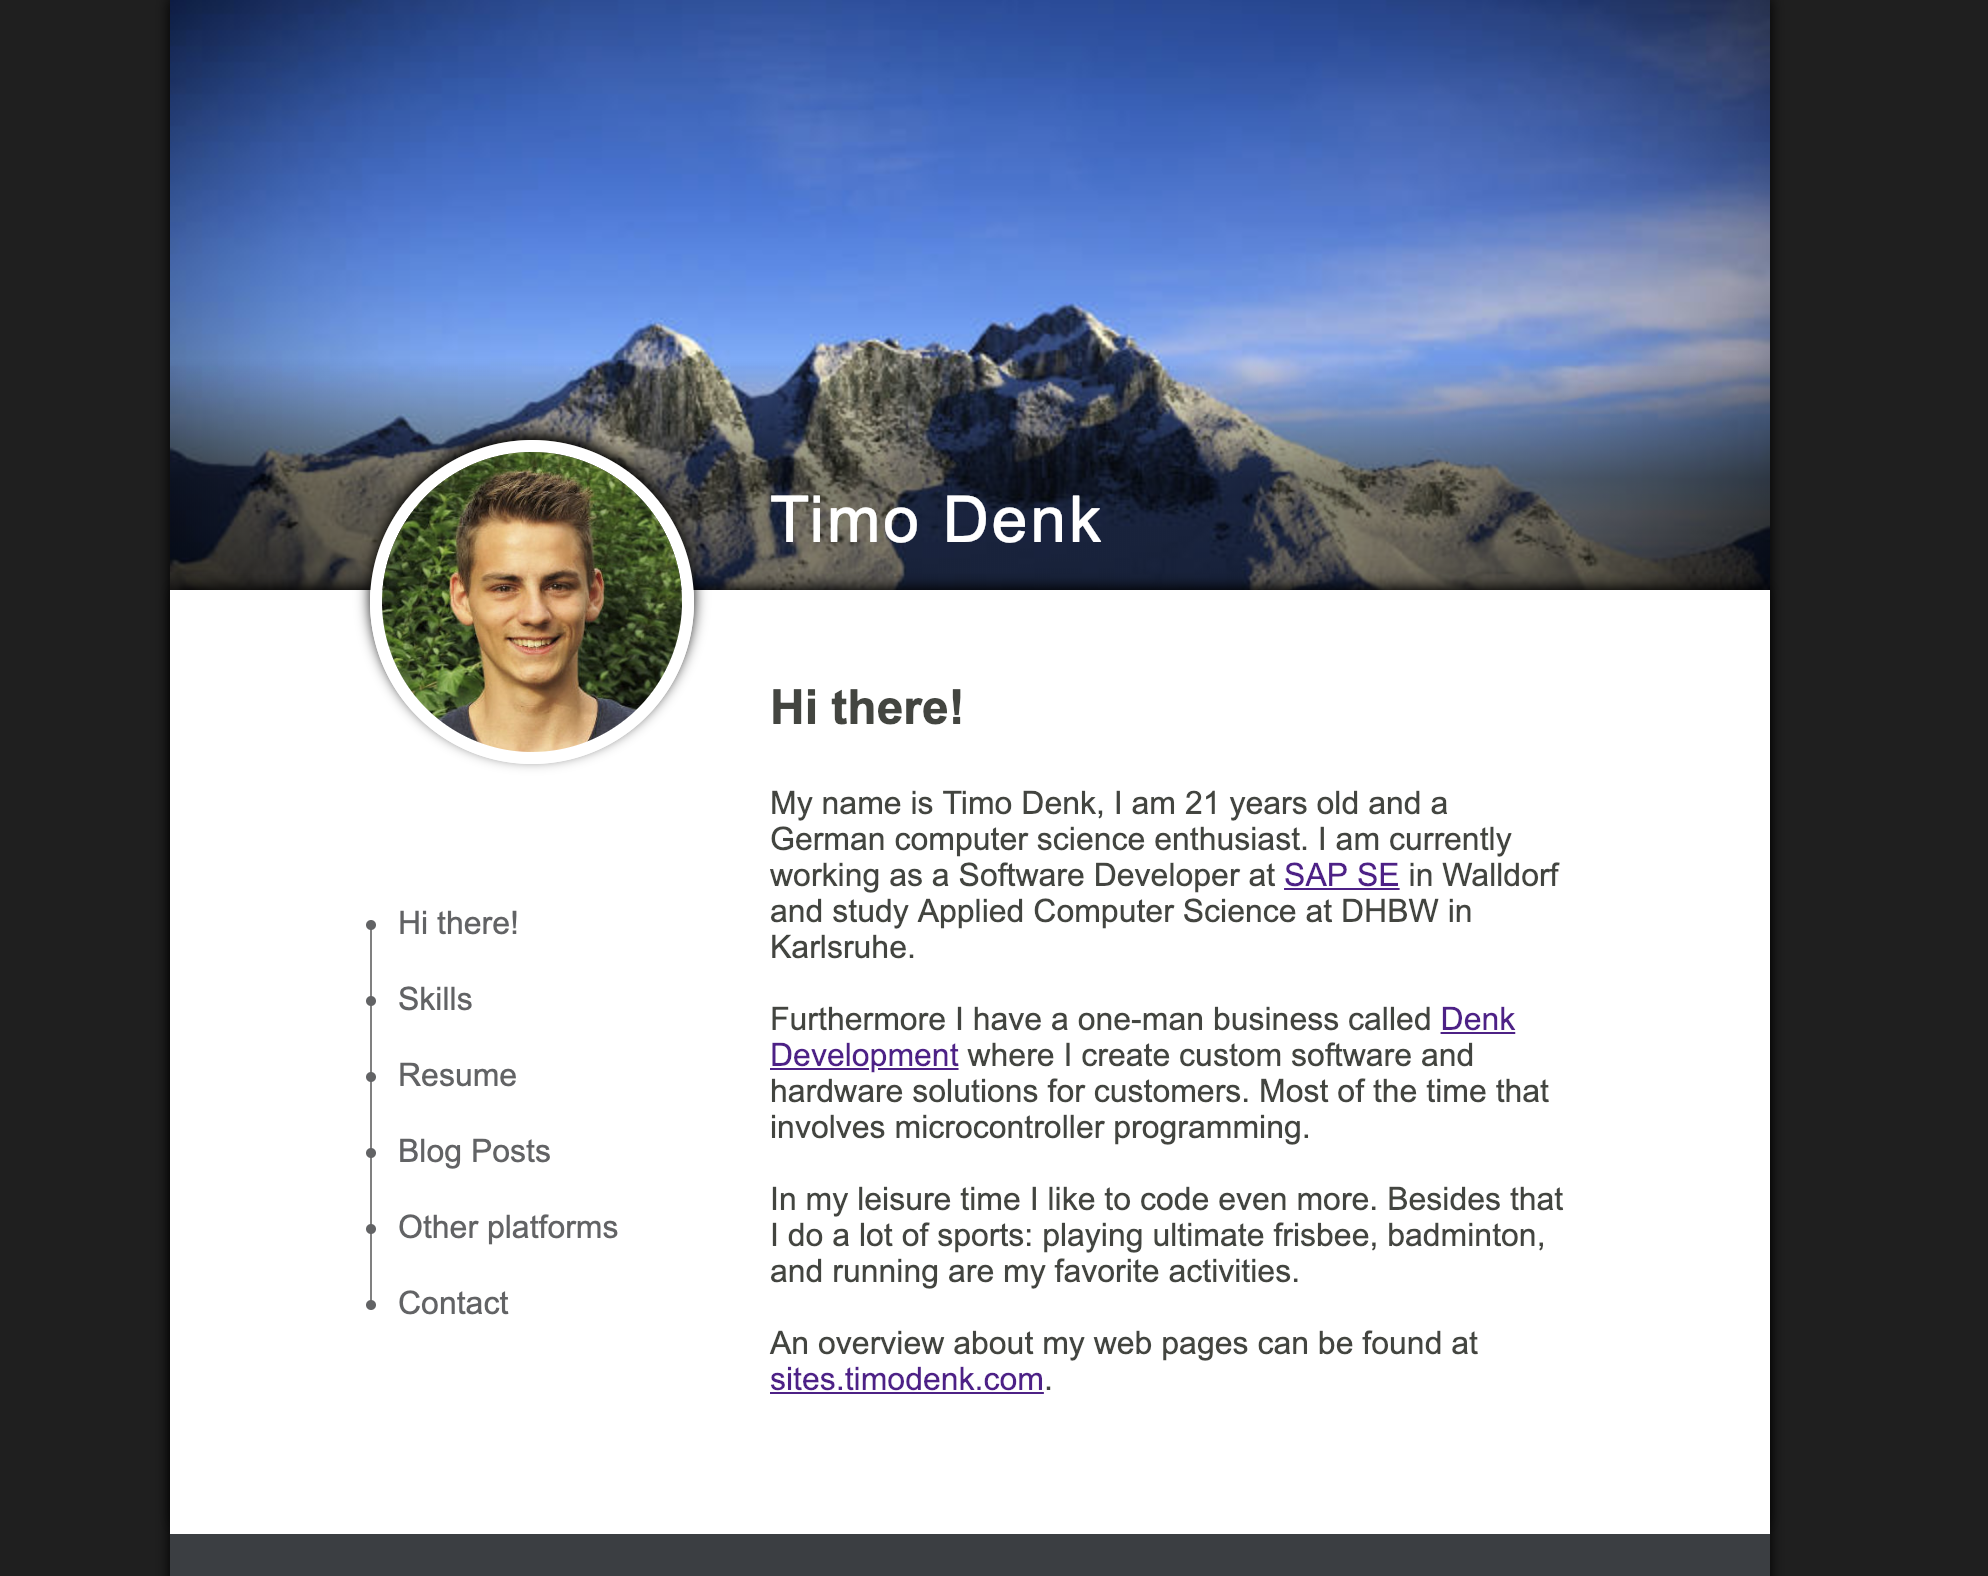
\includegraphics[width=.5\textwidth]{resources/timodenk}
	\nodepart{three} 
\includegraphics[width=.25\textwidth]{resources/timodenk_mobile}
	\nodepart{four} Timo Denk
	\nodepart{five} 636 ms
	\nodepart{six} 434 kb
};

\node[vertices]  (sites) at (10,2) {
\nodepart{one} \texttt{sites.timodenk.com}
\nodepart{two} 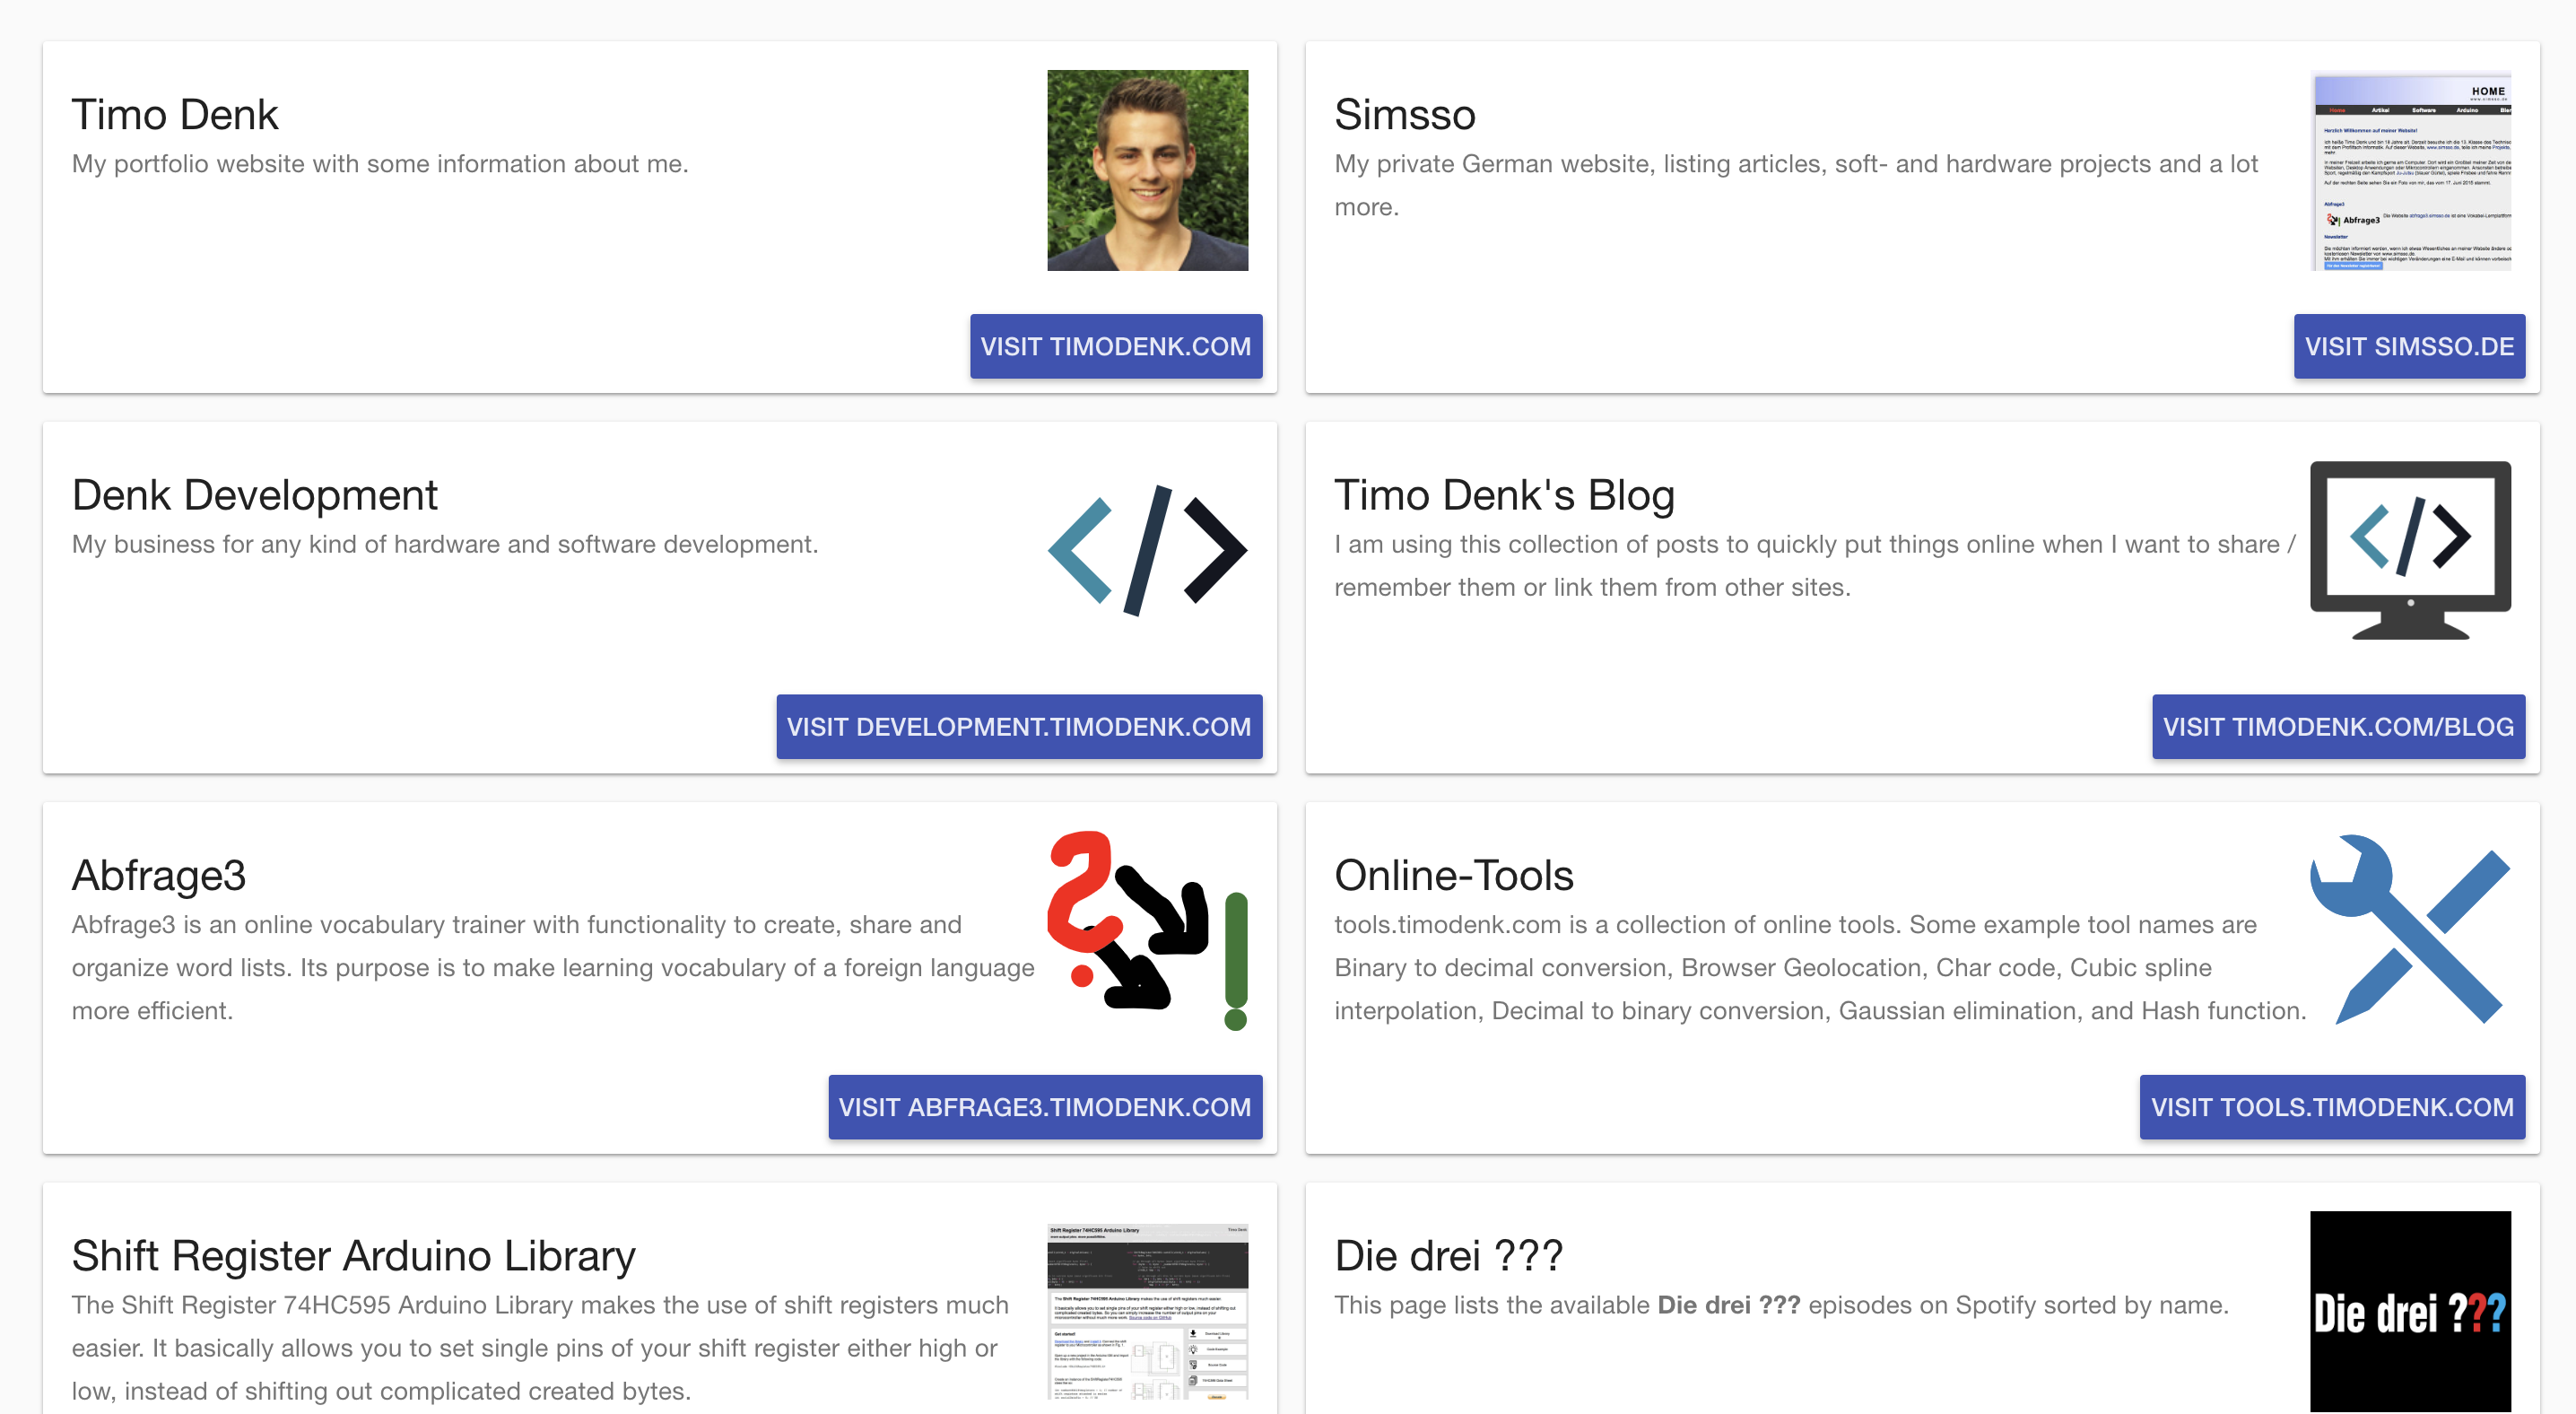
\includegraphics[width=.5\textwidth]{resources/sites_timodenk}
\nodepart{three} 
\includegraphics[width=.25\textwidth]{resources/sites_timodenk_mobile}	\nodepart{four} Timo Denk Sites Overview
\nodepart{five} 767 ms
\nodepart{six} 737 kb
};

\node[vertices]  (imprint) at (0,2) {
\nodepart{one} \texttt{timodenk.com/imprint}
\nodepart{two} 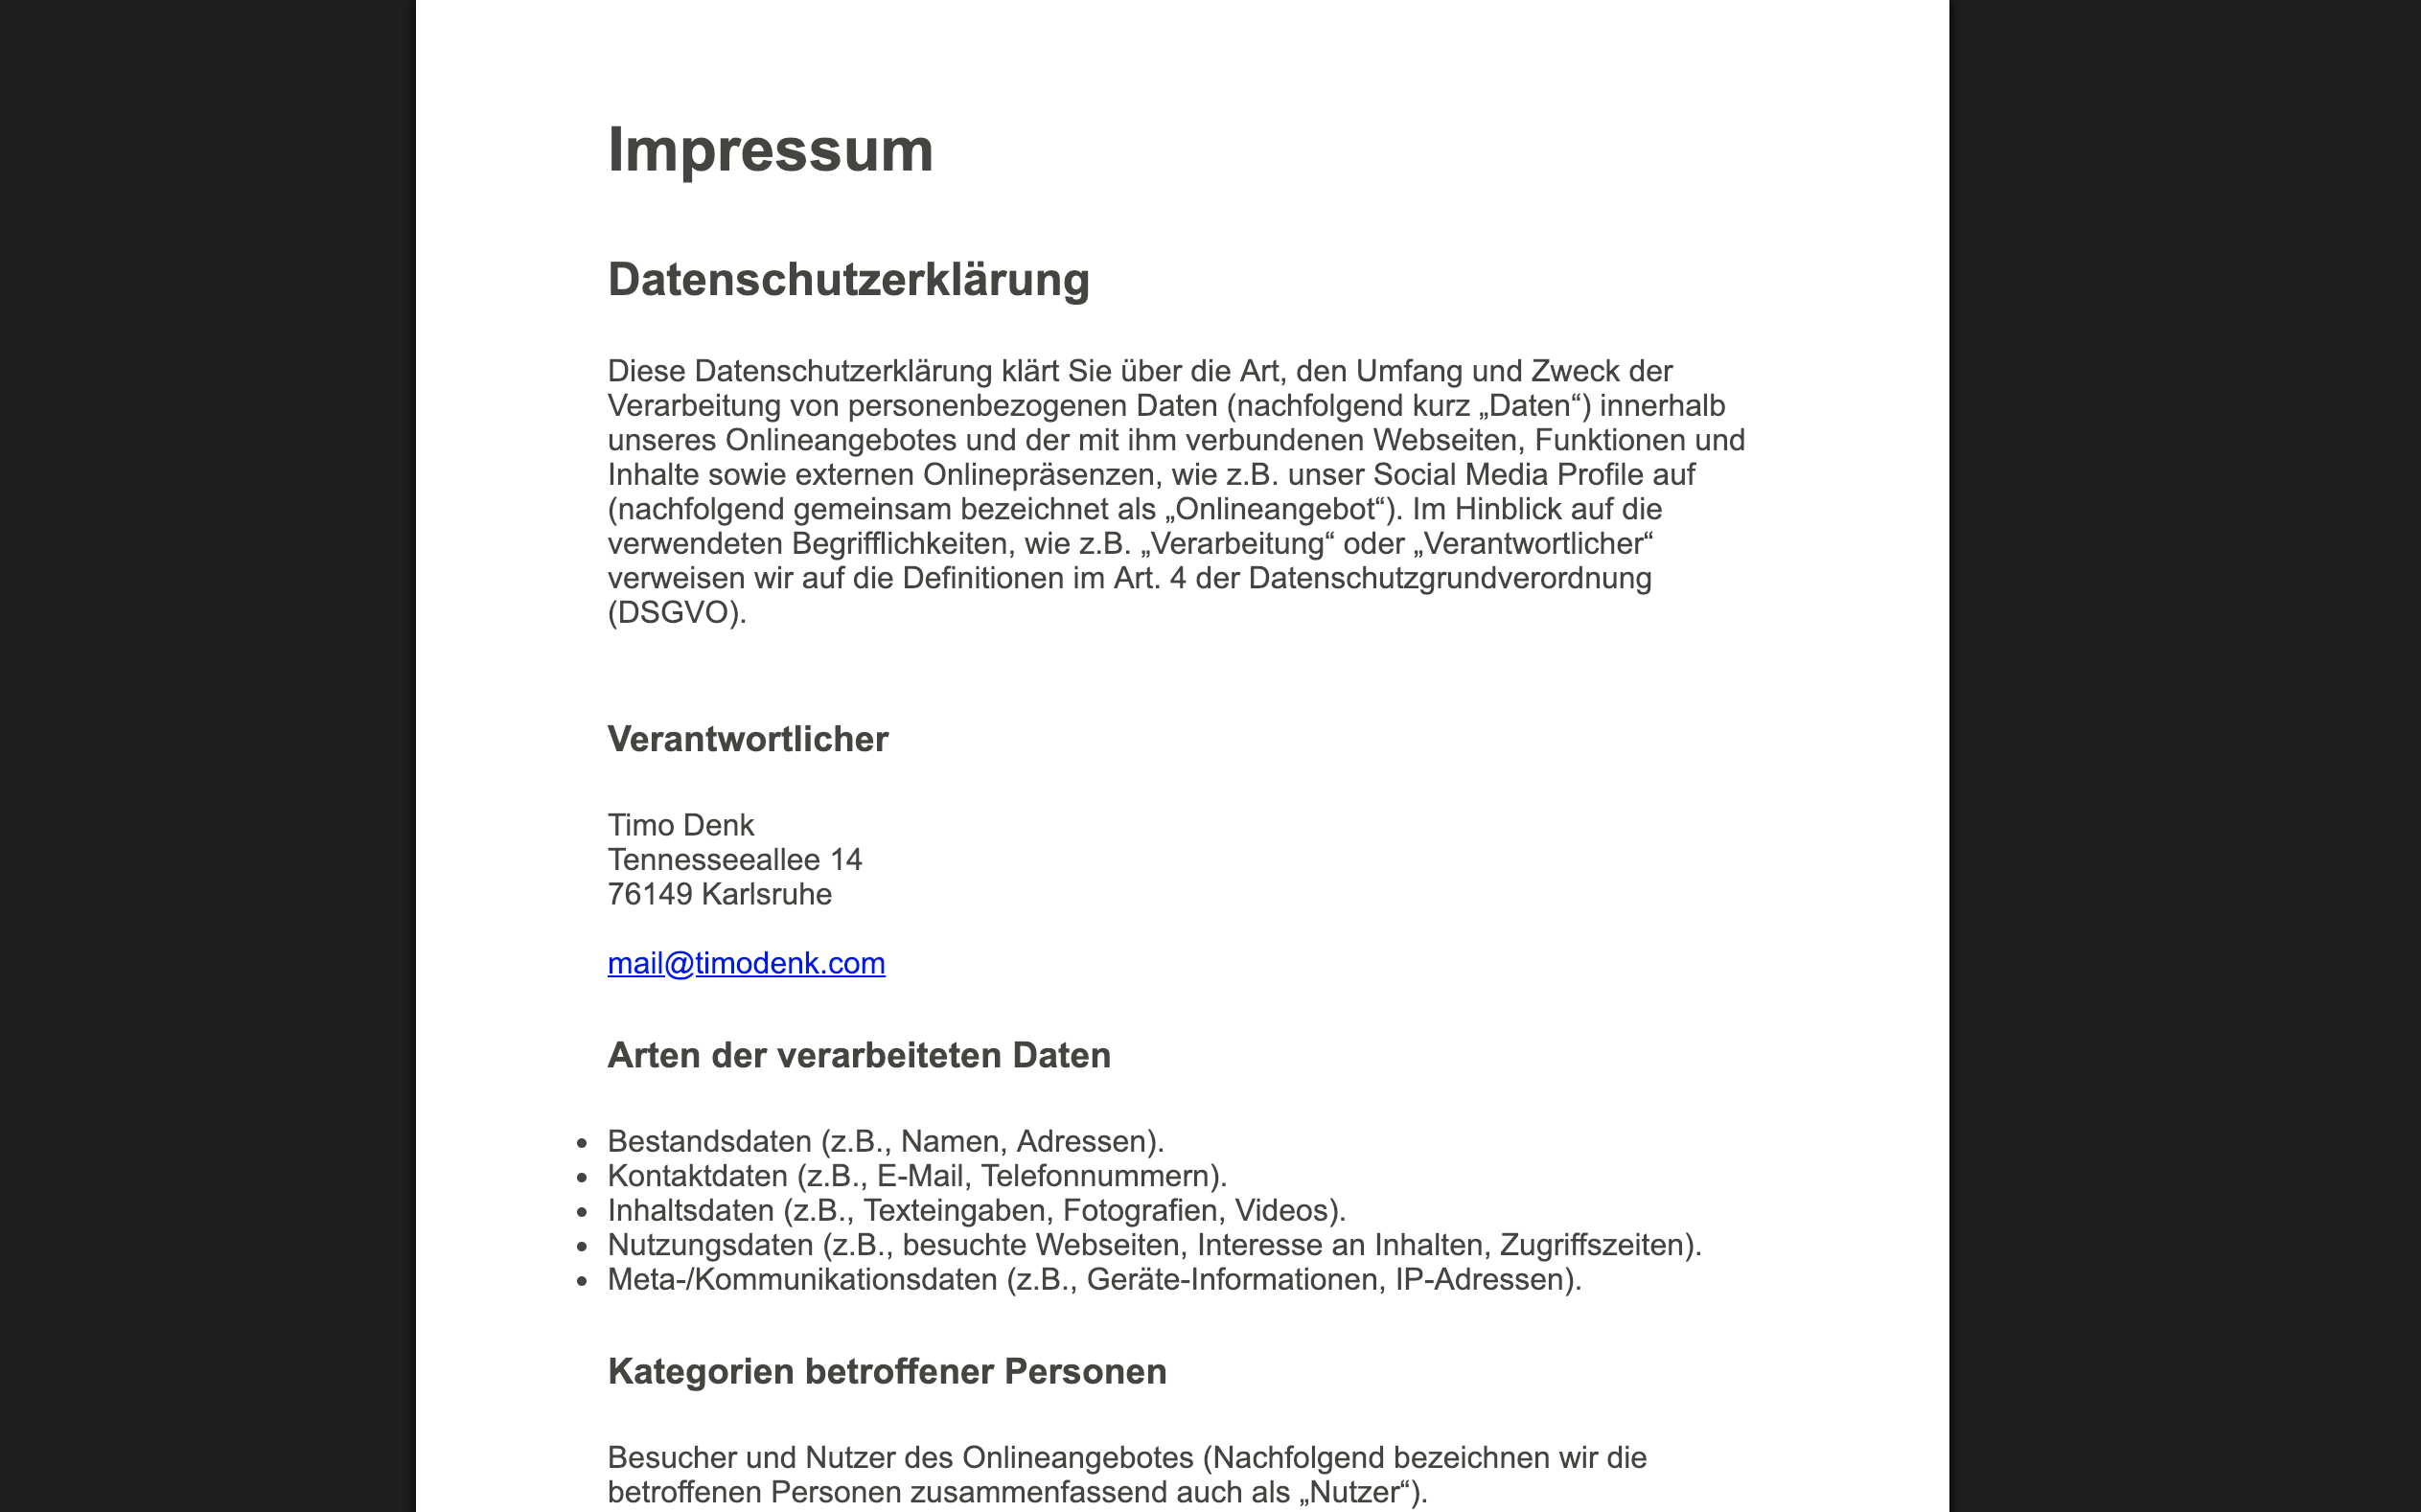
\includegraphics[width=.5\textwidth]{resources/imprint_timodenk}
\nodepart{three} 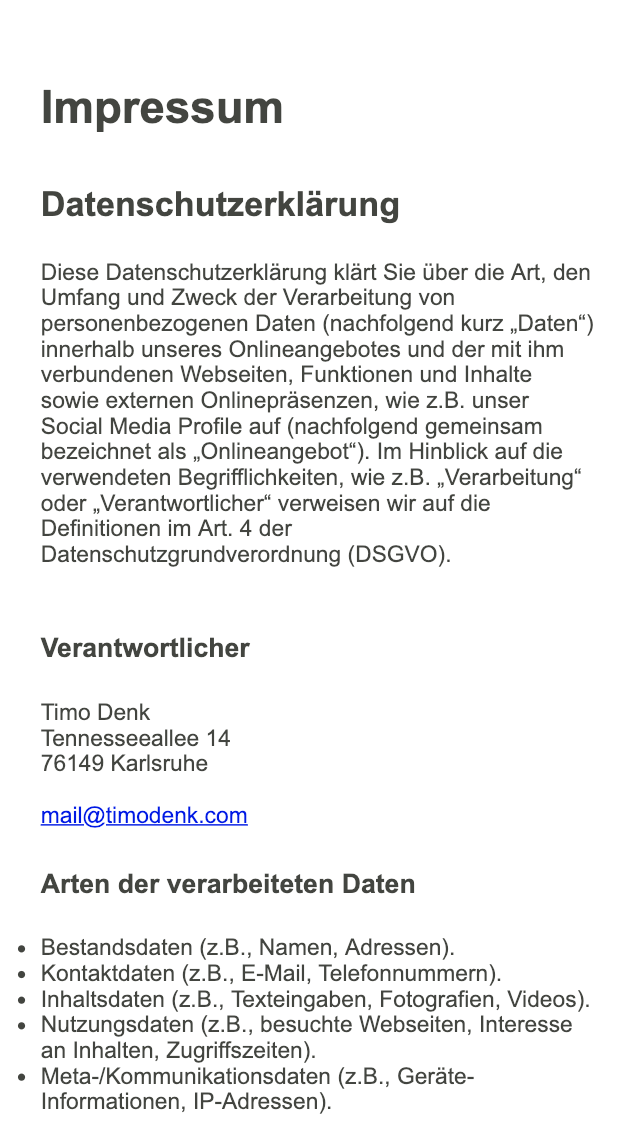
\includegraphics[width=.25\textwidth]{resources/imprint_timodenk_mobile}
\nodepart{four} Imprint - www.timodenk.com
\nodepart{five} 304 ms
\nodepart{six} 52 kb
};

\node (timodenkToImprint) at (0.5,6) {\texttt{timodenk.com/imprint}};
\node (timodenkToSites) at (9.5,6) {\texttt{sites.timodenk.com}};
\node (SitesToTimodenk) at (5.5,0.25) {\texttt{timodenk.com}};
\draw[-latex] (timodenk.one east) to [bend left=30] (sites.one north);
\draw[-latex] (sites.six west) to [bend left=30] (timodenk.six south);
\draw[-latex] (timodenk.one west) to [bend right=30](imprint.one north);
\end{tikzpicture}
}
\caption{Illustrates partial directed graph of domain \texttt{timodenk.com} with three web pages, corresponding arrows and vertices}
\label{fig:PartialDirectedGraph_timodenk.com}
\end{figure}
